%design session experience
During previous co-designing events researchers have  experienced limited ability among COPD-patients to interact with co-designing tools due to the physical limitations of their disease. While conversing some patients are even not able to participate in other activities \citep{genTech}. Based on these experiences we scaled down our initial idea of the patient as an active partner in a co-designing event. We made a concise plan where patients only were expected to either talk or interact with a prototype. To further reduce the workload on the patients, we gave/sent each patient a workbook with minor assignments for completion over three days prior to the actual design session. The idea with the workbook was to spread out work from the design session on more days, freeing up time for talking and sharing thoughts during the session and sensitize the patients to the topic, promote reflection about collection and reflection. Initially we wanted to develop a prototype with them, but with the co-designing experience from \citep{genTech} we decided to developed a prototype that simulates our proposal of a telehealth system, which the patients could try and criticize. Ideally we wanted to gather all the patients in one room for a common design session but since the patients are less mobile and easily gets tired, the sessions were conducted as individual sessions in the patients' own homes. We used the same COPD-patients as in study one, which enabled us to ask some follow-up questions that had arisen since study one. However one patient was hospitalized and could not participate meaning the study included five COPD-patients.

\section{The Workbook}

The workbook assignments dealt with collection, data reliability and reflection. We wanted to know more on how patients collect objective and subjective data (both in relation to binary and granulated subjective questions). We also wanted to know if patients understand the meaning of the values and while collecting reflect on whether the readings are reliable and if they repeat measures. We wanted to see if selected binary subjective measures were based on estimation or recall. Further, we wanted to know if visualizing measures relative to a normal area trigger any reflection and if access to previous subjective measures (both  binary and granularity) affect the assessment. We therefore made assignments to all these areas and we also included measuring assignments to include their personal measures in the prototype. The workbook is included on attached CD.


\section{The Prototype}

Our proposal for the telehealth prototype contains three types of pages. 1) Collection, a page for entering measures, 2) Visualisation, a page for seeing past measures and 3) Dashboard, a page for fast (not detailed) visualisations of the data, giving current state, e.g. downward and/or upward trends of the measures.

\textit{add 1, Collection:}

In \ref{fig:colObj} and \ref{fig:colSubj} we have examples of the objective and subjective collection page (respectively).
Both types of the collection pages (subjective and objective) have a reference graph in the top, which shows previous measures. We think, by giving a reference graph, current state can easily be compared with previous measures, which could help judging upward or downward trends. We hope, by knowing previous subjective measures a better consistency across measures will occur. As literature suggest, annotation can foster reflection, we therefore have a note area in the bottom of both types of pages (subjective and objective), where the patient can add further reasoning, e.g. "my oxygen supply is 2" or "I just started the ventilation system, it is so hot, hopefully it will make my breathing easier". Above the note area, we have toggle buttons of context variables that the patient can toggle on/off if he thinks one/or more is relevant. Hopefully, the context variables makes casual explanation easier and starts reflection. Depending on type of collection page (subjective or objective), the page contains check-boxes to provide a subjective measure or a text-field to provide an objective measure.


\begin{figure}[h]
  \centering
  \begin{minipage}[b]{0.45\textwidth}
    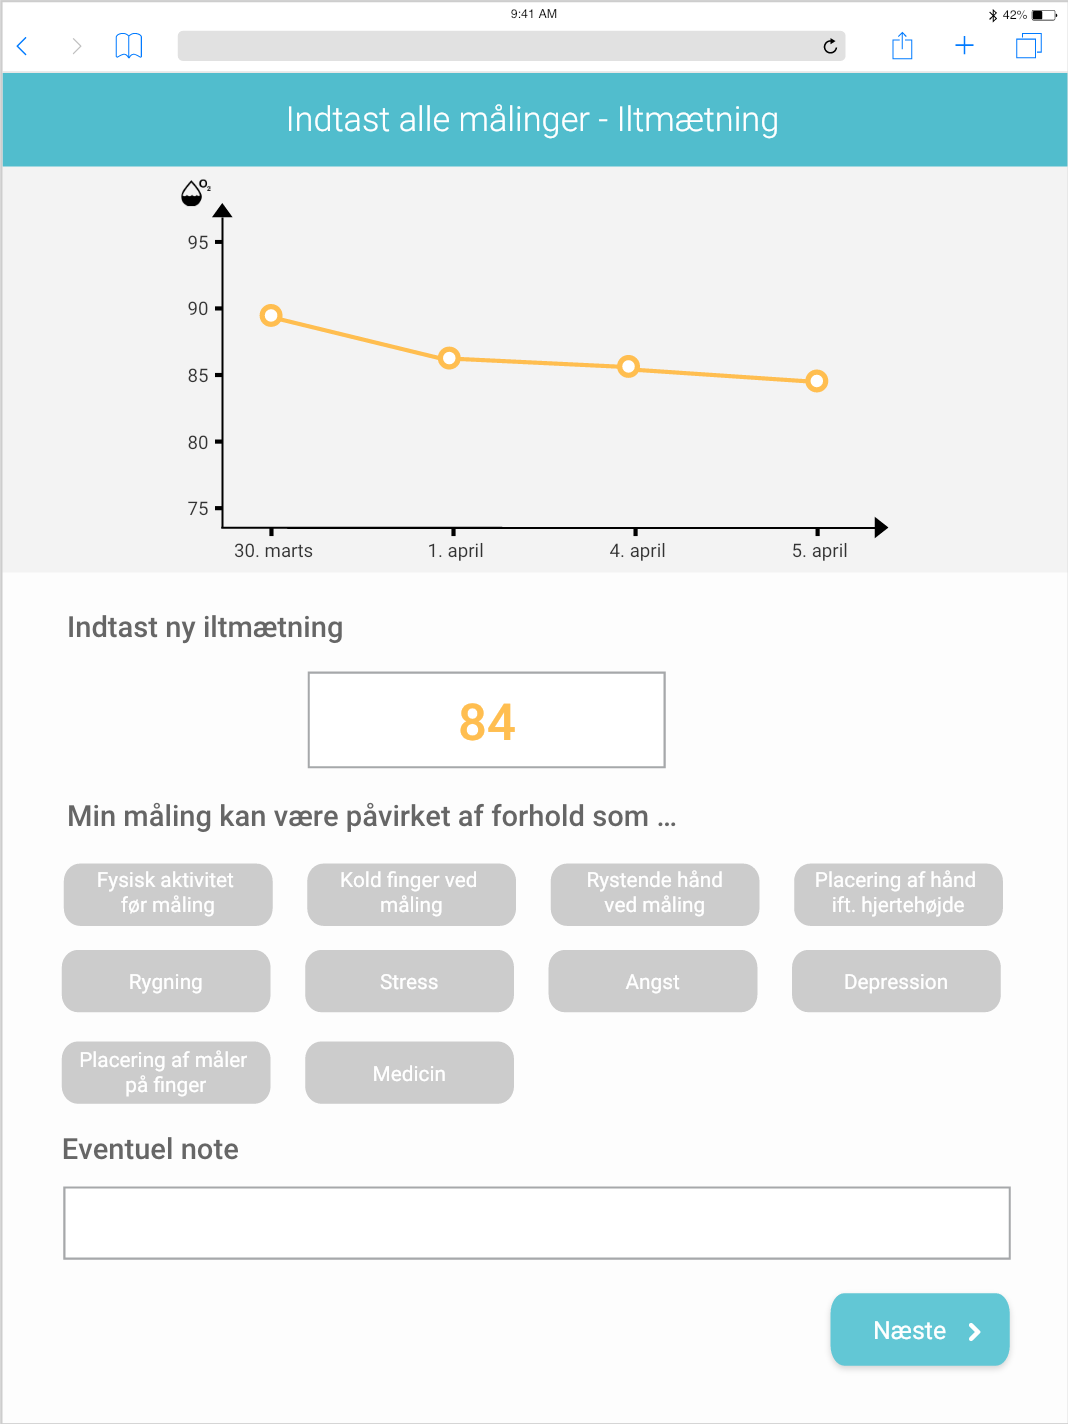
\includegraphics[width=\textwidth]{images/study2/collectionObj.png}
    \caption{Shows the user Interface for collection of objective measure (in this example saturation).}
    \label{fig:colObj}
  \end{minipage}
  \hfill
  \begin{minipage}[b]{0.45\textwidth}
    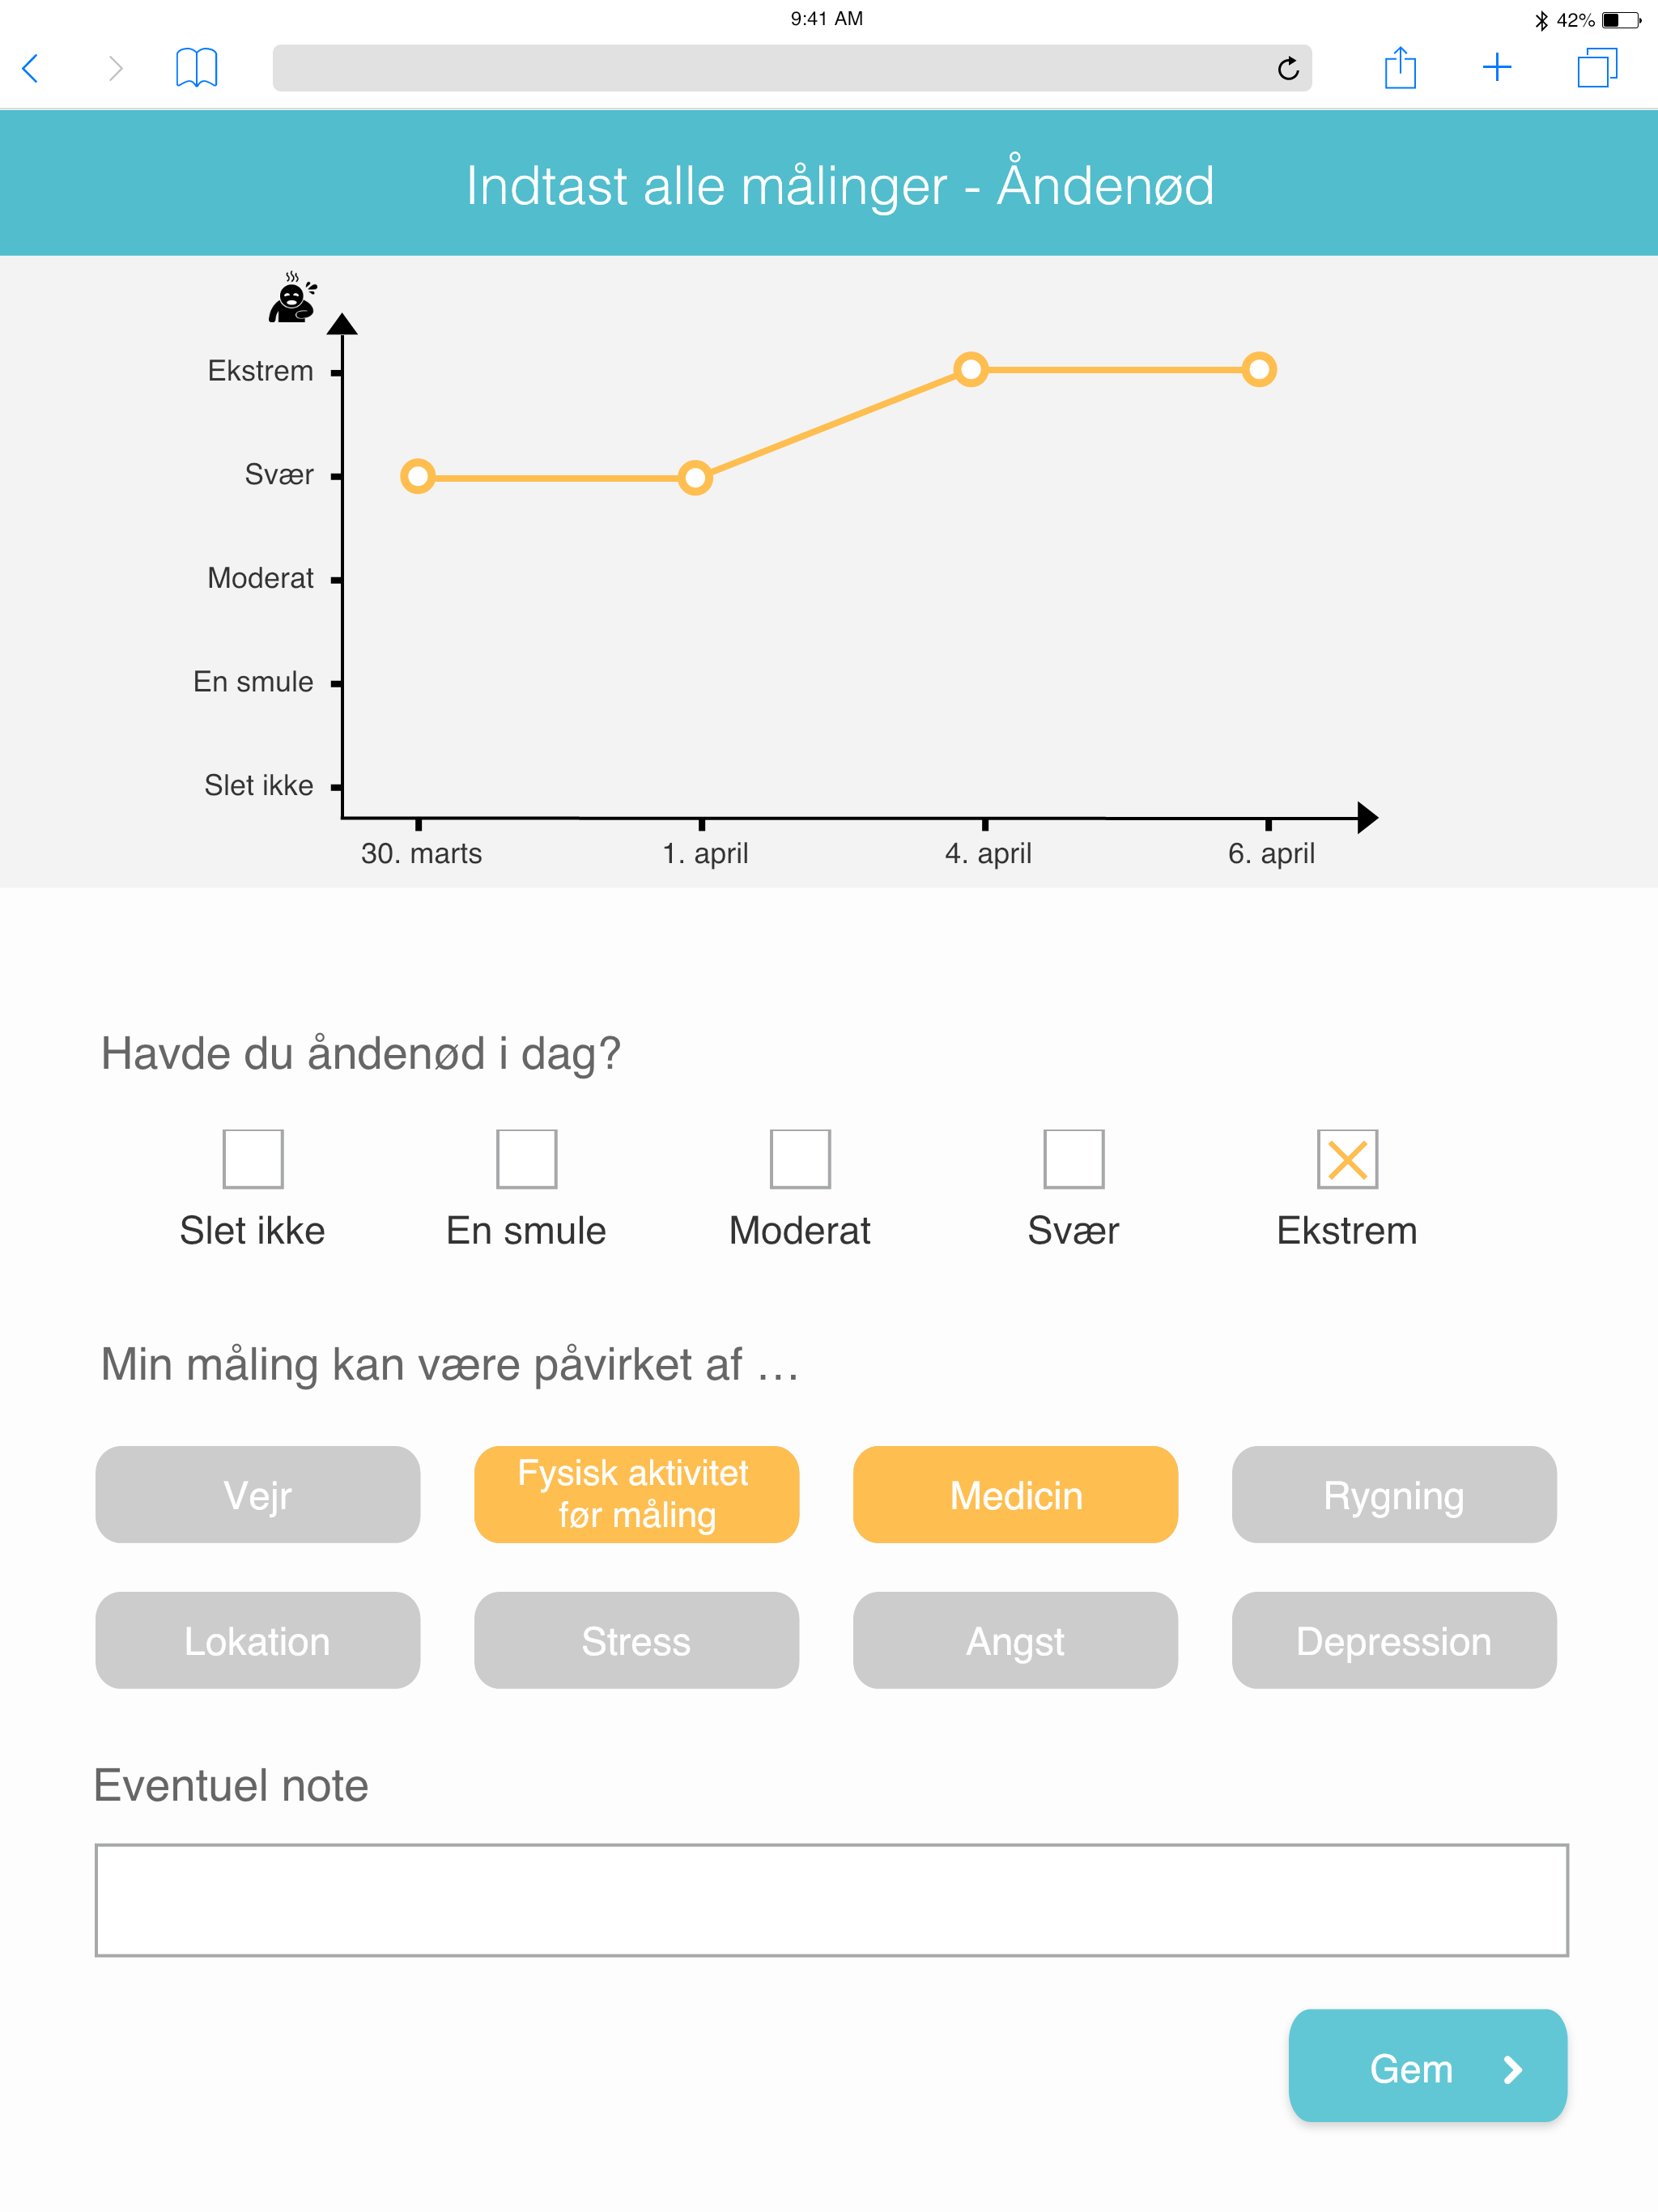
\includegraphics[width=\textwidth]{images/study2/collectionSub.png}
    \caption{Shows the user interface for collection of subjective measure (in this example dyspnea).}
    \label{fig:colSubj}
  \end{minipage}
\end{figure}

The prototype was developed in Adobe Experience Design and the project can be found on detached CD as well as an example url to the running prototype.

\textit{add 2, Visualisation:}

We included interactive visualisations of previous measures to facilitate long-term reflection. We developed four types of visualisations and wanted to see, which one the patients' preferred. 

In terms of facilitating the identification of temporal location and quantitative value of a particular data point, the authors of "Investigating time series visualisations to improve the user experience" found that users prefer visualisations with clear textual tooltips over highlighting. Their finding also indicated tooltips as more effective than highlighting and that cartesian coordinate system in general is comparable or more effective than Polar coordinate system. They also found that interactive time series visualisations enhances the user experience \citep{adnan2016}.
% except when searching for a minima. 

The authors of the paper "Financial Visualization Case Study: Correlating Financial Timeseries and Discrete Events to Support Investment Decisions" find visualising discrete events on time series problem-free only when multiple discrete events visually do not overlap and when the visualisation of the discrete event does not overlap an axis which holds important information (e.g. price). They also present an alternative visualisation if wanting to visualise multiple discrete events simultaneously, which has proved successful in practice \citep{sorenson2013}.

Based on these two papers we included interactive time series, containing textual tooltips in different types of cartesian coordinate systems. Discrete events are visualised one type at a time (when toggled) to avoid overlapping. We also included a calendar heatmap to support the visualisation of human behaviour, which often are characterized by periodic patterns \citep{Cuttone}. The calendar heatmap is also interactive and shows discrete events with same functionality as just described, see figure \ref{fig:v4}. 

\begin{figure}[h]
  \centering
  \begin{minipage}[b]{0.45\textwidth}
    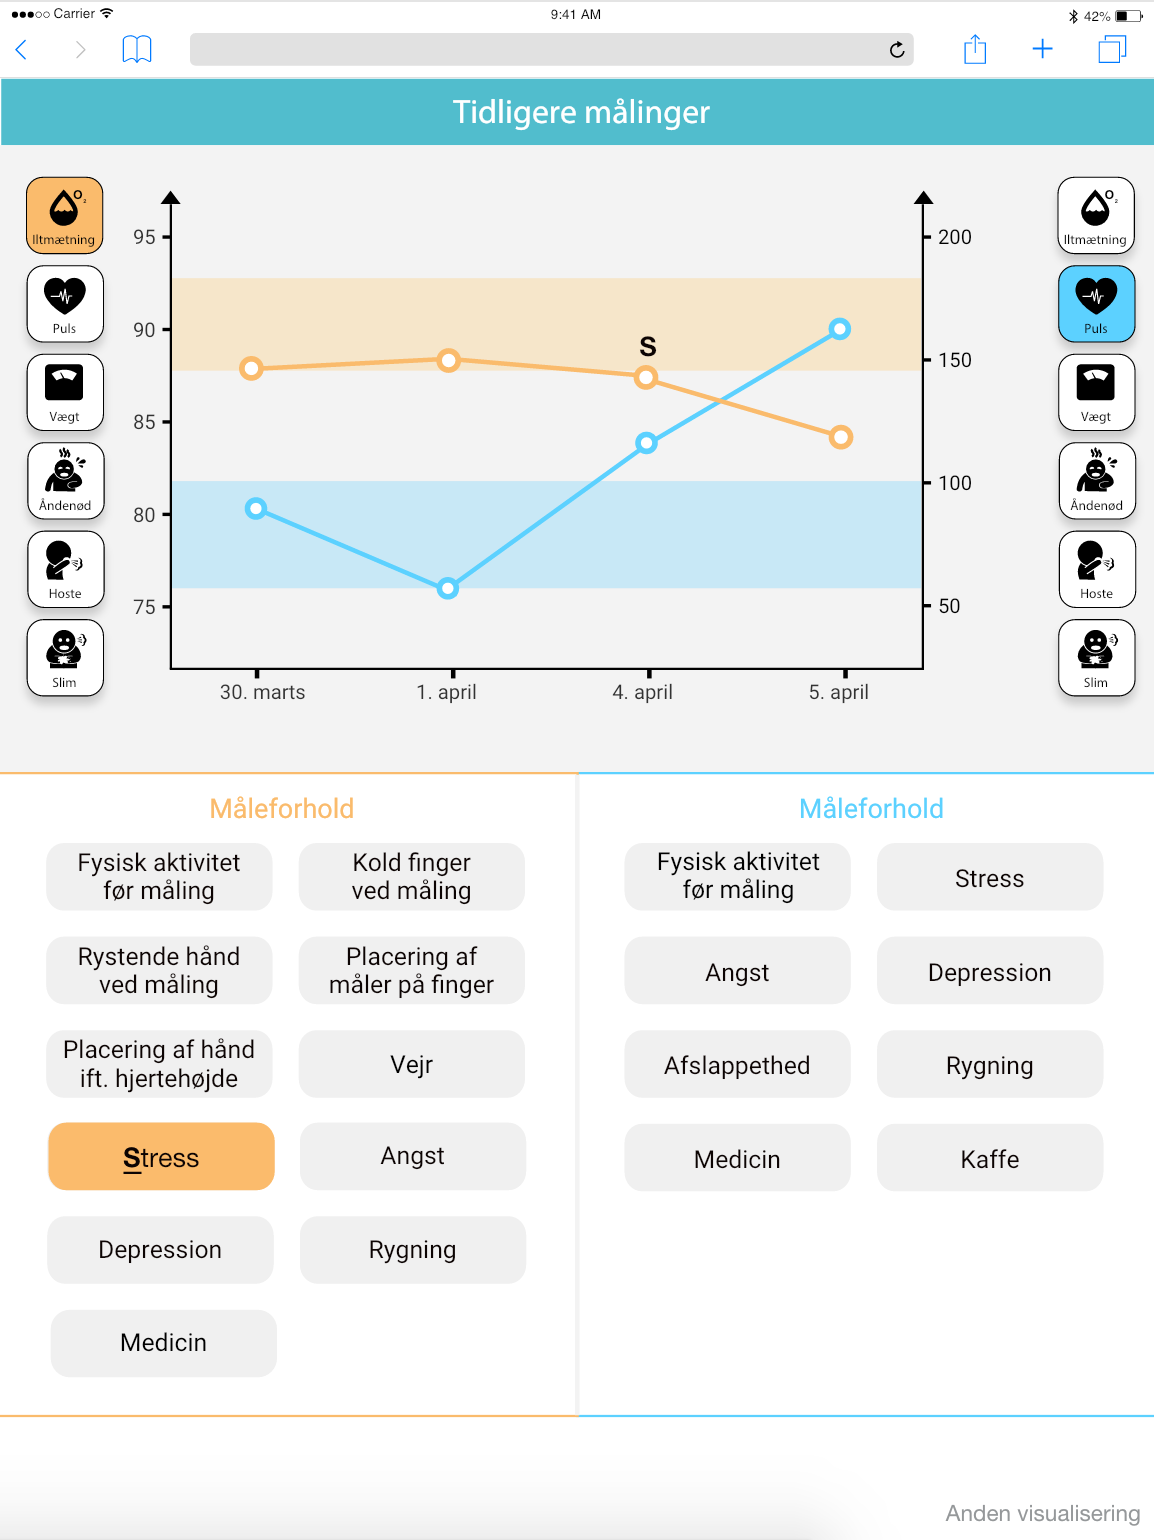
\includegraphics[width=\textwidth]{images/study2/v1.png}
    \caption{Visualisation 1.}
    \label{fig:v1}
  \end{minipage}
  \hfill
  \begin{minipage}[b]{0.45\textwidth}
    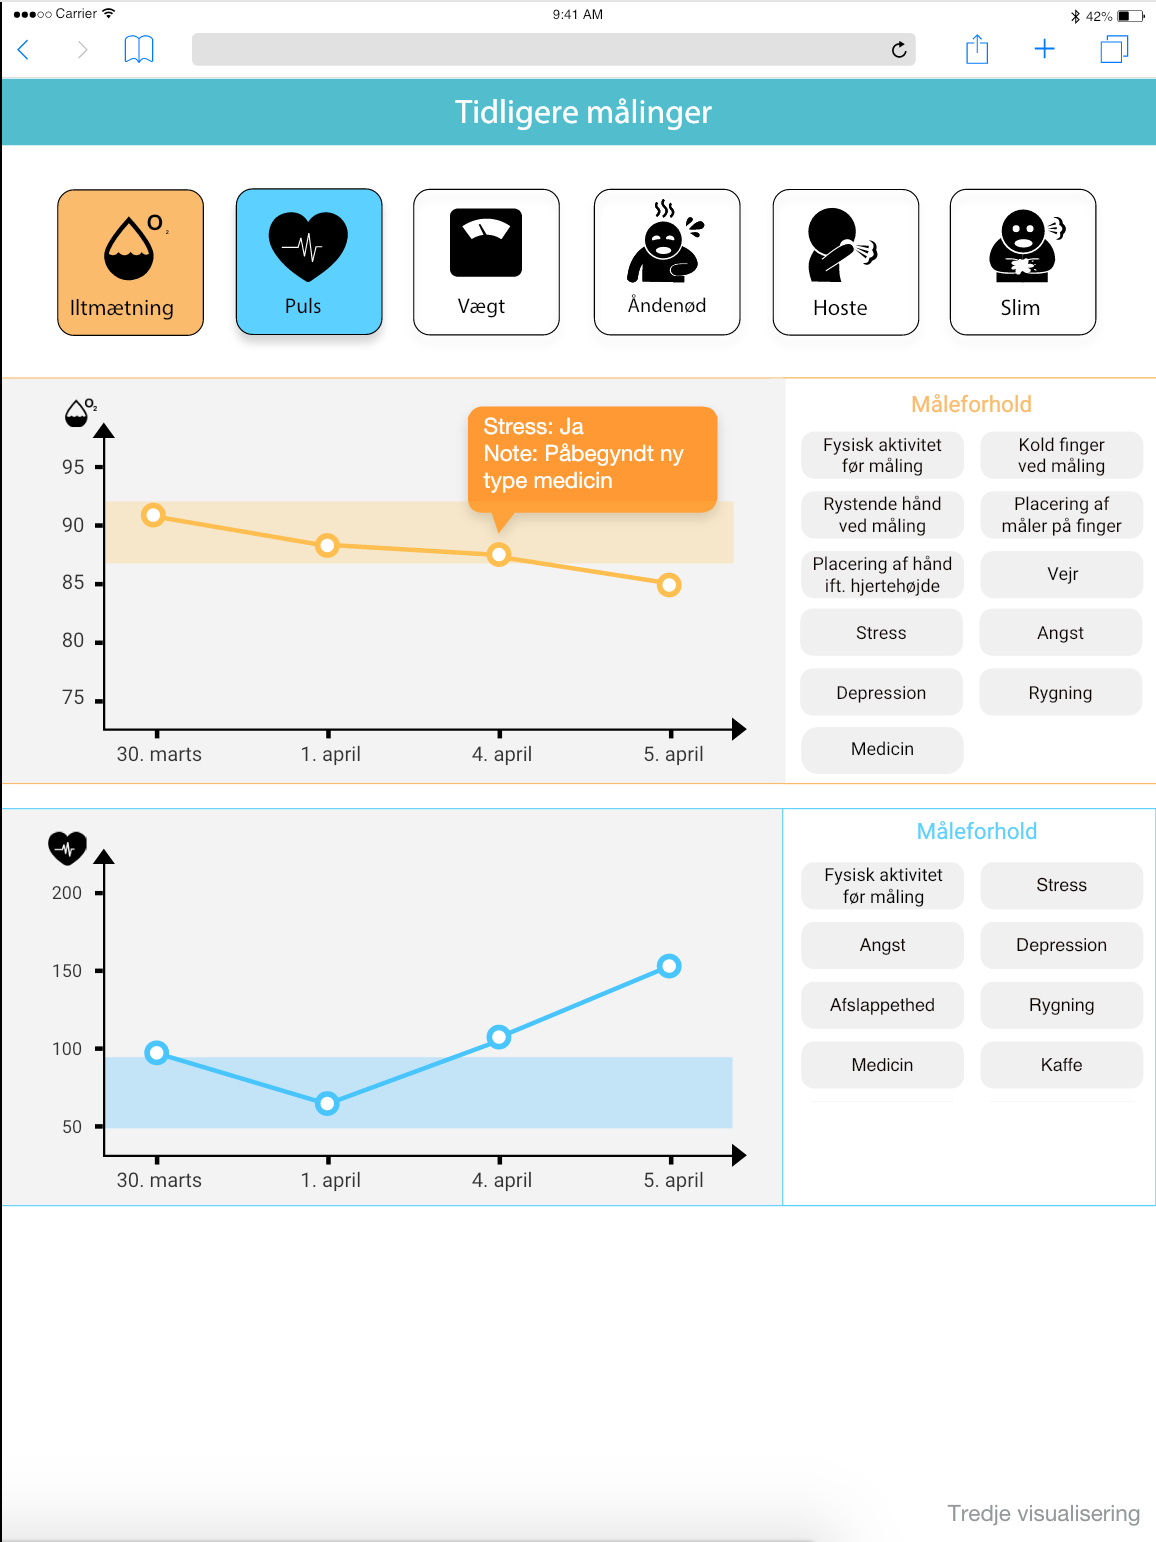
\includegraphics[width=\textwidth]{images/study2/v2.png}
    \caption{Visualisation 2.}
    \label{fig:v2}
  \end{minipage}
\end{figure}

\begin{figure}[h]
  \centering
  \begin{minipage}[b]{0.45\textwidth}
    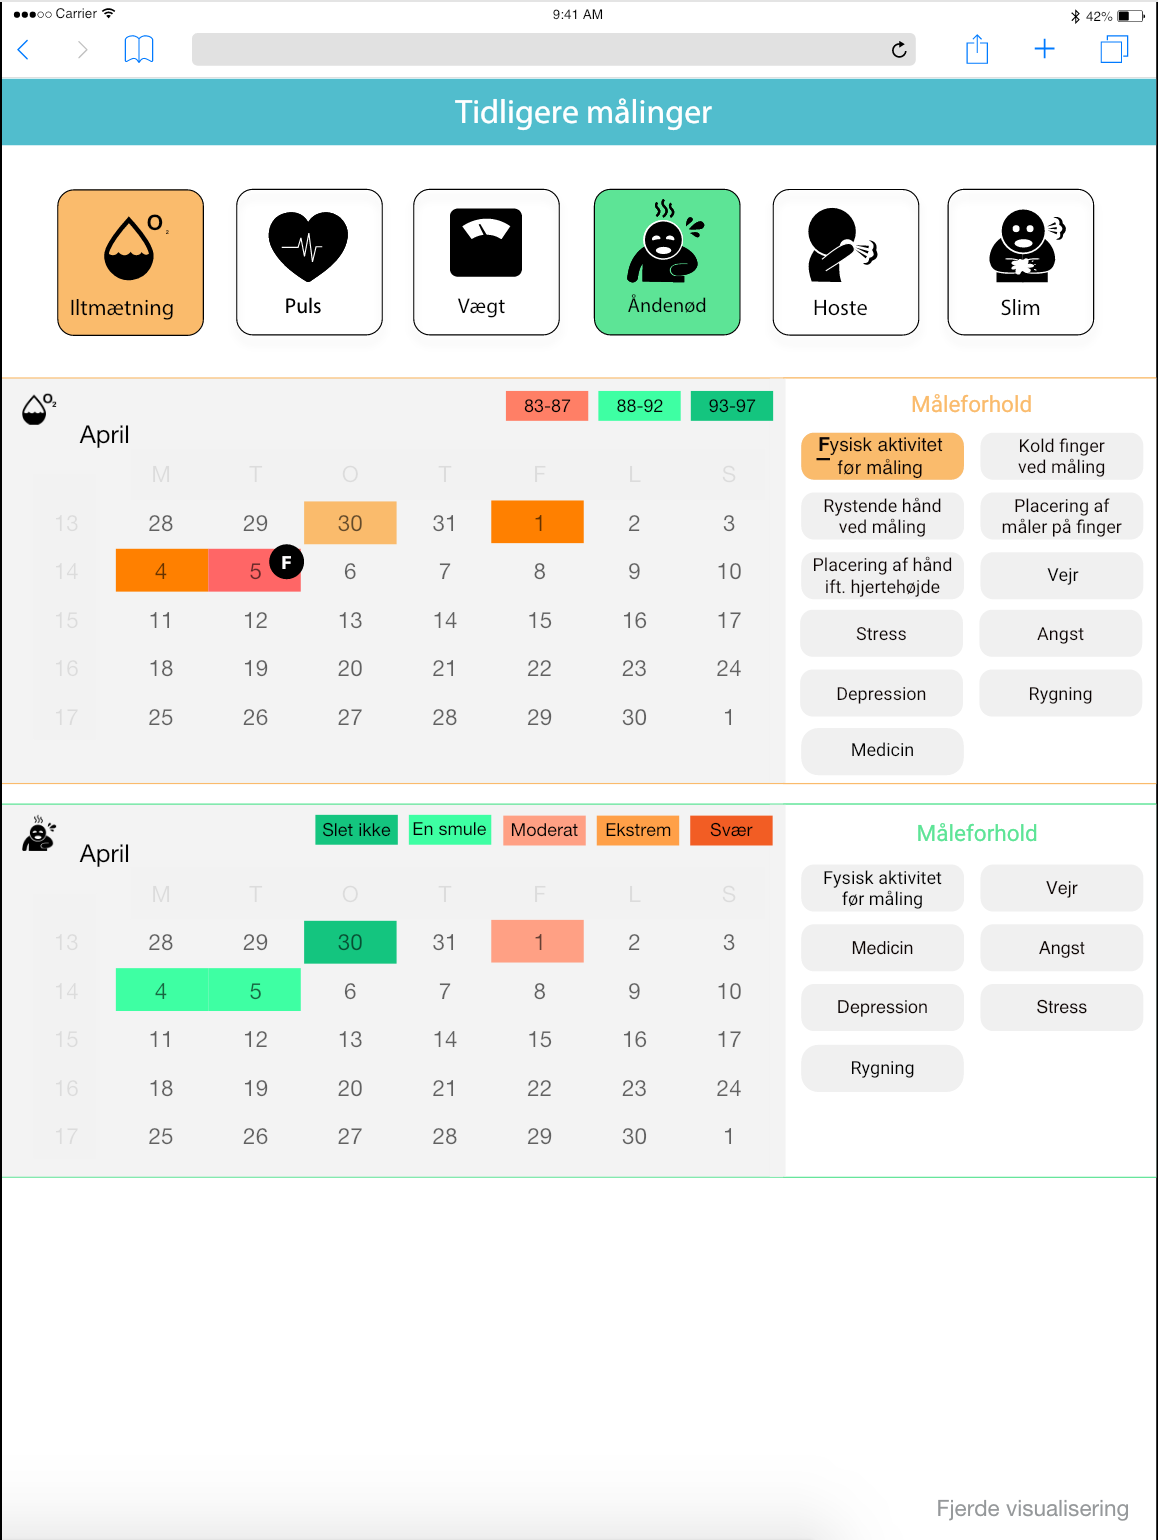
\includegraphics[width=\textwidth]{images/study2/v3.png}
    \caption{Visualisation 3.}
    \label{fig:v3}
  \end{minipage}
  \hfill
  \begin{minipage}[b]{0.45\textwidth}
    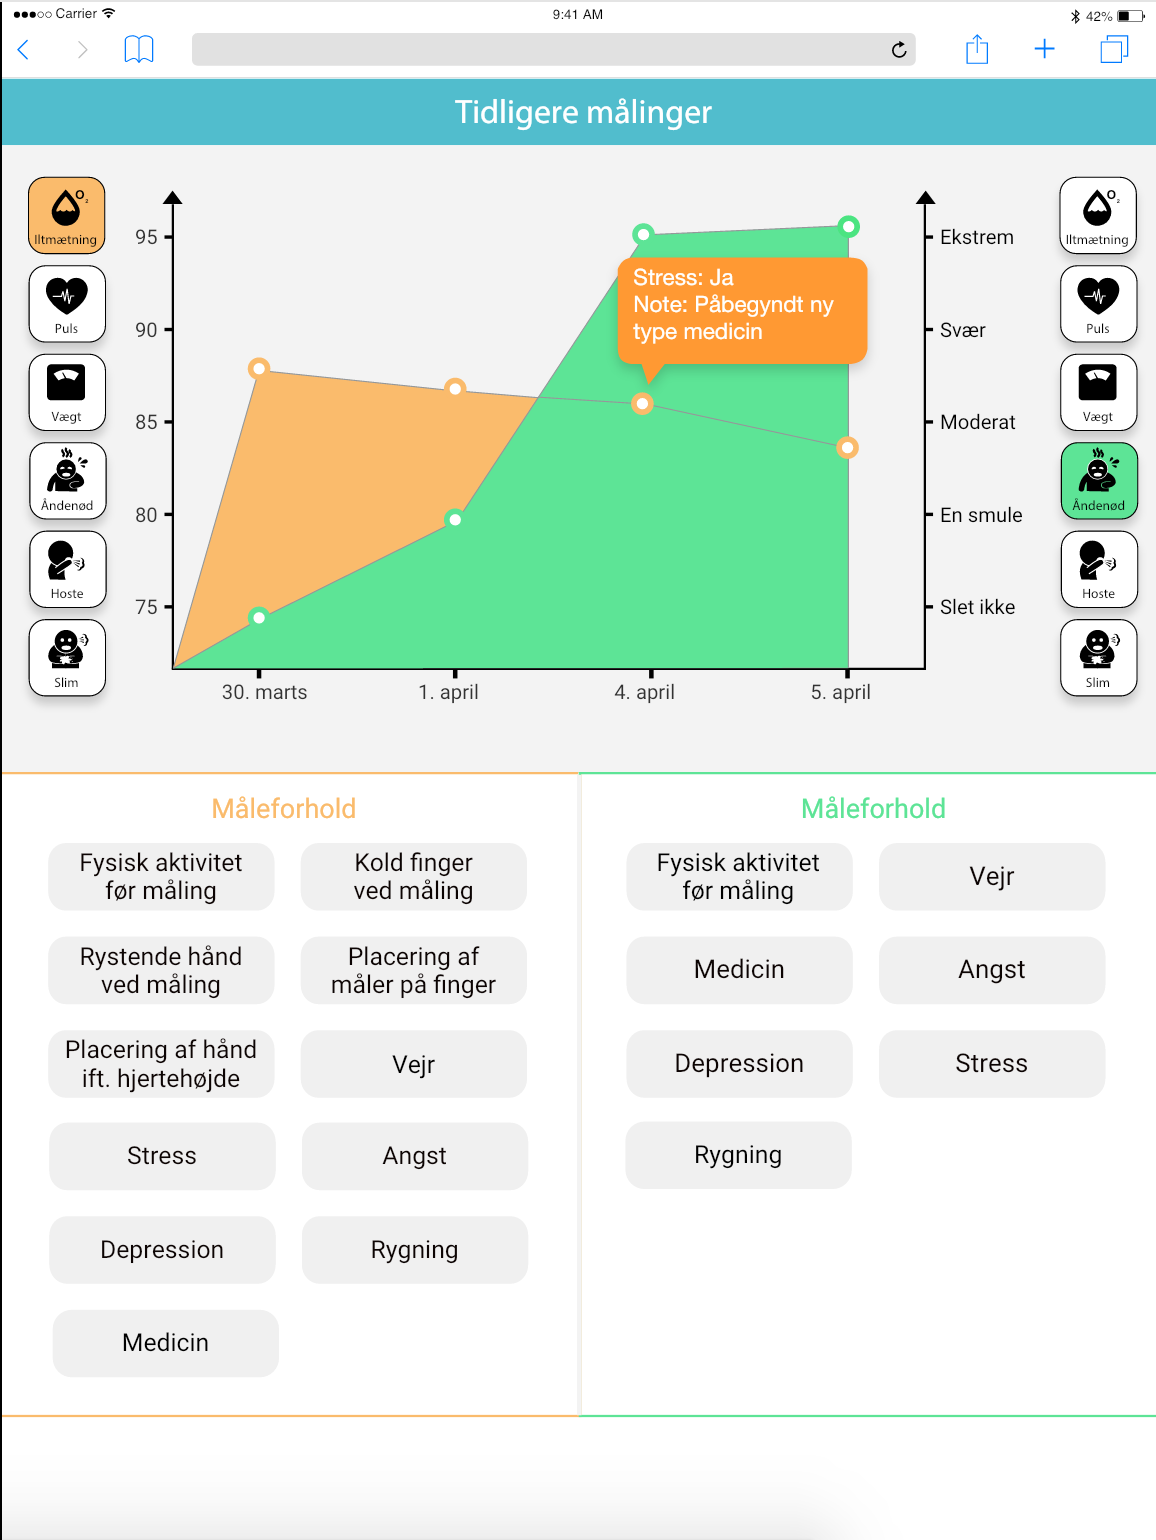
\includegraphics[width=\textwidth]{images/study2/v4.png}
    \caption{Visualisation 4.}
    \label{fig:v4}
  \end{minipage}
\end{figure}

\FloatBarrier

\textit{add 3, Dashboard:}

The dashboard supports short-term reflection by showing current state relative to normal areas by color coding and upward/downward trends with use of arrows. We also included reflective questions written in orange in relation a measure, see fig \ref{fig:dashboard}.

\begin{figure}[h]
\centering
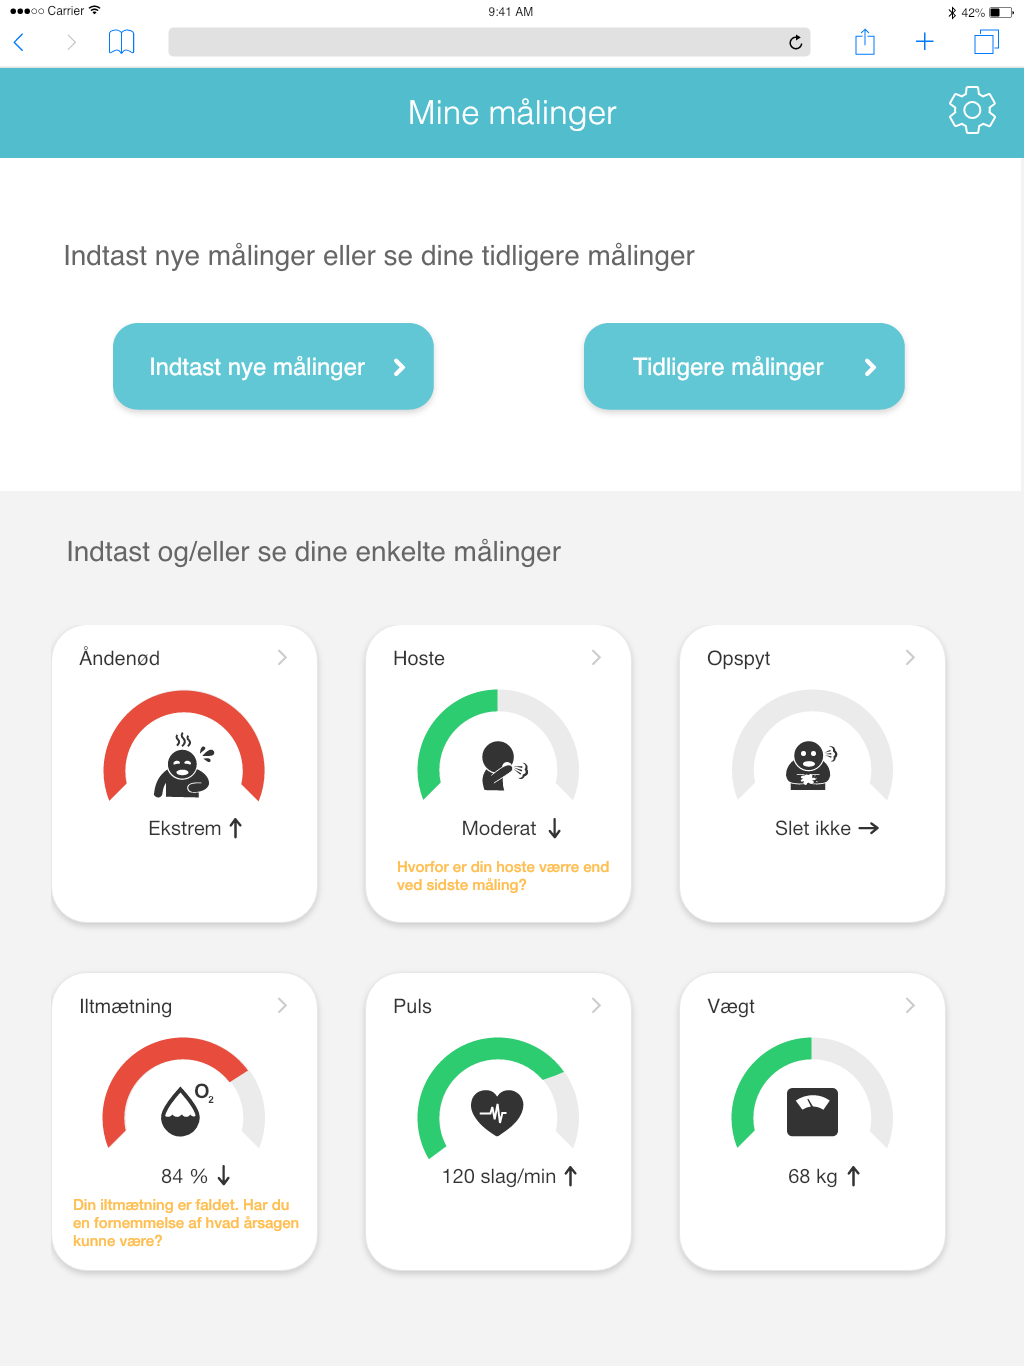
\includegraphics[scale=0.18]{images/study2/Dashboard.png}
\caption{The dashboard.}
\label{fig:dashboard}
\end{figure}

\FloatBarrier

\section{Activity Plan}

We here bring the activity plan from the study.

\textbf{Agenda:}
\begin{itemize}
\small \item Consent form (included on attached CD)
\item Part one - Follow-up questions from first visit
\item Part two - Workbook
\item Part three - Prototype 
\end{itemize}

\textit{Process:}

Two researchers were present during each session. The researcher that facilitated study one continued the interview from last time with the follow-up questions while the other researcher prepared part two by looking through the patient's workbook. During part two the first researcher prepared the prototype by adding in personal measures from the patient's workbook in the prototype (sometimes this process was done right before the session if the researchers arrived early to the patient's house).

\textit{Data collection:}

We audio recorded the whole design feedback session. During the prototype part we used UX Recorded for iOS to record the screen, the front camera and the audio. The recordings are all to be found in detached CD.


\textbf{Part 1 - Follow-up}

Time:
\begin{itemize}
\item How long time have you used Tunstall Healthcare and/or AmbuFlex?%Hvor lang tid har du brugt Tunstall og/eller Ambuflex? Eller en anden telemedicinsk løsning?
\item How long time do you spend on measuring and sending data through  AmbuFlex to the hospital?%Hvor lang tid bruger du på at måle og sende data ind til hospitalet?
\item How much time are you willing to spend on measuring and sending data?%Hvad er din smertegrænse?
\item How long time did it take to learn to use AmbuFlex?%Hvor lang tid har du brugt på at lære at bruge AF?
\item How does the weather influence your COPD (if it influences)? %Hvordan påvirker vejret din KOL, hvis den gør?
\end{itemize}

Guidelines:
\begin{itemize}
\item Have you been taught how to do correct measures? (e.g. when to use the saturation device?) %har du fået vejledning i hvordan du tager korrekte målinger?
%Fx. hvornår saturationsmåler skal bruges? (fysisk tilstand)
\end{itemize}

Collection phases:
\begin{itemize}
\item How do you prepare for using the pulse oximeter?%kan du fortælle mig, hvordan du gør dig klar til at foretage dine målinger og hvad du gør? (før)
\item Would you like to have access to your previous measures?%Kunne du tænke dig at have adgang til dine tidligere målinger? 
\end{itemize}

Reflection:
\begin{itemize}
\item Anything specific you need to better reflect on your measures?%Noget specielt der skal til at for at du lettere kan reflektere over dine målinger?
\item Do you miss visualisations of your measures?%savner du visualisering/grafer?
\end{itemize}

In case the patient do parallel tracking:
\begin{itemize}
\item Have you improved your tracking system while tracking? %Har du løbende lavet det om, forbedret det?
\item What do you think of your own tracking system?%Hvad synes du selv om dit eget system?
\item Is there anything you miss?%Er der noget du mangler?
\item Is there something that could be easier?%Er der noget der kunne være lettere?
\end{itemize}

Other:
\begin{itemize}
\item In cases of exacerbation, do you start medication earlier when having telehealth?%Føler du at du får opstartet medicinering tidligere når du bruger TM?
\item What motivates you to use AmbuFlex?%Hvad motiverer dig til at bruge Ambu-Flex?
\end{itemize}

\textbf{Part 2 - Workbook}

Purpose: Feedback on improved collection and understanding of how it fosters reflection while collecting.

\begin{enumerate}
\item Discussion on time of measurement (afternoon or morning) - pros/cons
\item Discussion on use of context variables on page 4 + 10
\begin{enumerate}
	\item Identification of level(s) of reflection:
	\begin{enumerate}
		\item When annotating context-related variables in the comment boxes
		\item When checking context-related variables in the check-boxes 
	\end{enumerate}
	\item Discussion on differences between above-mentioned two methods in terms of use, reflection and preference
	\item Discussion on relevance (e.g. cold finger) and priority of variables. 
	\begin{enumerate}
		\item Were you aware that these context variables could influence your measure? Discussion on need for explanation on context-related variables (in guidelines) 
		\item Any new-found variables?
		\item Discussion on shorter versions 
		\item Subjective measure: Dyspnea
	\end{enumerate}
	\item Discussion on what the assessment was based on (recall or estimation). Identification of level(s) of reflection, when assessing:
	\begin{enumerate}
		\item Binary
		\item Granularity (5 ordinal categories)
		\begin{enumerate}
			\item How is it different from binary? Better/worse? Why?
		\end{enumerate}
		\item Numbers (presented in workshop)
		\item Visuals
	\end{enumerate}
	\item Comparison of above-mentioned methods
\end{enumerate}
\item Objective measure: Normal area
\begin{enumerate}
	\item Ask about previous experience with graphs (control)
	\item Identification of level(s) of reflection :
	\begin{enumerate}
		\item What thoughts did the graph trigger?
		\item How are you measurements in relation to the normal area? What do you think of that? What do you think of the normal area shown?
	\end{enumerate}
\end{enumerate}
\item About having a reference graph when assessing binary measures (Identification of level(s) of reflection)
\begin{enumerate}
	\item What thoughts did the graph trigger?
	\item How does it affect your answer to whether you feel more breathless than usual when you can see your previous answers?
\end{enumerate}
\item About having a reference graph when assessing more granular answers (Identification of level(s) of reflection)
\begin{enumerate}
	\item How does it affect your answer (to whether you felt breathless today) (assessed on 5-point), when you can see your previous answers?
	\item Is there any benefit in seeing your previous measures?
\end{enumerate}
\end{enumerate}


\textbf{Part 3 - Prototype}

Purpose: Primarily for usability purpose and feedback on visualisation part.

Dashboard:
\begin{itemize}
\item You are on the dashboard. What do you notice first?
\item What does the arrow besides your oxygen saturation measure tell you? What does the arrow besides phlegm tell you?
\item What does the status indicator besides oxygen saturation tell you?
\item How do you feel about the color indications on your health status?
\item Imagine that you want to input a single oxygen saturation measure. Show me what you would do. 
\end{itemize}

Collection: 
\begin{itemize}
\item You want to go back now. Show me what you would do.
\end{itemize}

Dashboard:
\begin{itemize}
\item You want to enter all your measurements. Show me what you would do. (OBS: In this version you will only be able to enter two measures.)
\end{itemize}

Collection
\begin{itemize}
\item You have taken your saturation measure and it is 84 today. Enter it in the system.
\item You want to take the next measurement. What do you do now?
\item You had extreme shortness of breath today. Enter it in the system.
\item Mark that you have taken your medicine that affects your shortness of breath. Then mark that you have been physical active.
\item You want to save your measurement.
\item Do you want to send your measurement to the hospital? If yes, proceed.
\end{itemize}

Dashboard:
\begin{itemize}
\item Now you are back on the dashboard.
\item Now you want to see all your previous measures. What do you do?
\end{itemize}

Visualisations:

\textit{\small Visualisation 1}
\begin{itemize}
\item You see the graph of your oxygen saturation. You also want to see dyspnea, what do you do?
\item Instead of dyspnea, you know what to see cough, what do you do?
\item You want to see when stress has affected your oxygen saturation measures. What do you do?
\item What do you think about this visualisation? What do you notice on this visualisation?
\begin{itemize}
 \item Identification of level(s) of reflection
 \end{itemize}
\end{itemize}



\textit{\small Visualisation 2}
\begin{itemize}
\item You see the graph for your oxygen saturation. You also want to see dyspnea, what do you do?
\item You also want to see pulse. What do you do?
\item You want to remove the graph for dyspnea. What do you do?
\item You want to see more details on the oxygen saturation measure made on the 4th of April. What do you do?
\item What do you think about this visualisation? What do you notice on this visualisation?
\begin{itemize}
	\item Identification of level(s) of reflection
	\end{itemize}
\end{itemize}

\textit{\small Visualisation 3}
\begin{itemize}
\item You see the graph for your oxygen saturation. You also want to see dyspnea, what do you do?
\item You want to see whether physical activity before the measure has influenced your saturation. What do you do? 
\item What do you think about this visualisation? What do you notice on this visualisation?
\begin{itemize}
	\item Identification of level(s) of reflection
	\end{itemize}
\end{itemize}

\textit{\small Visualisation 4}
\begin{itemize}
\item You see the graph of your oxygen saturation. You also want to see dyspnea, what do you do?
\item You want to see more details on the oxygen saturation measure made on the 4th of April. What do you do?
\item What do you think about this visualisation? What do you notice on this visualisation?
\begin{itemize}
	\item Identification of level(s) of reflection
	\end{itemize}
\end{itemize}

Other questions
\begin{itemize}
\item Visualisation of weather. How does weather affect you?
\item Currently, you share your measures with the hospital. Imagine a system, where it is not required. Can you imagine you entered measures, but did not want to share them with the hospital? Why/why not?
\end{itemize}



\section{Post Methodological Considerations}

When considering the methods used from this study in a retro-perspective light we have gained new experience.  We used Adobe's brand new prototype tool Experience Design. Even though the process of developing the prototype was streamlined (only showing few limitations) we discovered some limitations related to the context of our use. The tool did not provide us with an off-line functionality, which meant that we needed to use our mobile hotspot from our phones in order to conduct the prototype parts. At one patient we even needed to connect to her Wi-Fi due to slow hotspot connection. Sometimes we  experienced lack and delays while having good hotspot connection because the software loads a lot of assets per view. This sometimes frustrated patients, which made them doubt in either the prototype's functionality or whether they were interacting in the right way (and therefore also doubted their own skills). On use, we concluded, that Adobe Experience Design is a good tool with limitations when using it in the field. 

We had hoped to gain more knowledge from the workbooks but there was a mismatch between our expected user needs and the user's actual needs. Many assignments related to the time series, which most patients were not interested in reflecting on. In the workbook, we asked if the time series activated any thoughts. We could have asked into feelings generated by the time series, which potentially could have generated different answers.

Having both audio recordings and video recordings (of screen and front camera) from part two (prototype) was redundant. The patient interacted with the iPad in such a way, that the front camera did not capture facial expressions (the iPad was typically placed on a table and not hold). The video recording added new information to the audio recording by showing which element the patient tried to interact with, which from the audio recordings often was clear.